\documentclass[journal, a4paper]{IEEEtran}

%\usepackage{cite}     
\usepackage{graphicx}   
%\usepackage{psfrag}   
%\usepackage{subfigure} 
\usepackage{url}      
%\usepackage{stfloats}  
\usepackage{amsmath}  
%\usepackage{array}


% Your document starts here!
\begin{document}

% Define document title and author
	\title{Species Identification with Deep Convolutional Networks}
	\author{Fabian Otto
	\thanks{Advisor: Dr.~Anirban Mukhopadhyay, GRIS, TU Darmstadt, SS 2018.}}
	\markboth{Seminar Visual Computing}{}
	\maketitle

% Write abstract here

% Each section begins with a \section{title} command
\section{Scores}

%	% \PARstart{}{} creates a tall first letter for this first paragraph
%	This short summary includes the current results and performance for the Species data set. 
%	The goal was to predict the species of an animal, which was caught on a camera trap image.
%	Those images cropped at the bottom (65 px) and top (30 px) in order to remove time stamps and logos. 
%	In previous experiments, which maintained these parts of the image, the network was focusing on those parts in order to predict the species. 
%	For splitting the data into training and test data, a random stratified split was used in order to maintain the distribution of the dataset. 
%	Further, slight image augmentation is applied to generate a more robust model.
%	As model an (ImageNet) pretrained ResNet-50 Architecture was used and finetuned on the provided approximately 500.000 images. 
%	Due to the large amount of images supplied, experiments were also conducted with a ResNet-50 Architecture, which was trained from scratch, however, the results were significantly worse regarding both the training and the test accuracy.
%	Further, the val accuracy started to stall/decrease after training for only 5 epochs, learning rate adjustments did not overcome this issue as of now. 
%	Additional experiments, wich are still open, are larger Resenets as well as a better hyperparameter tuning and a class weighted training process. 
%	The latter was already started, but it seems that the network is focusing too much on infrequent classed, which simply represent noise.
	The currently best performing ResNet-50 Architecture achieves a test accuracy of 94.92\% and a corresponding training accuracy of 97.63\% after fine-tuning based on ImageNet for the provided Species data set.
	The accuracy`s improvement throughout the training progress can be seen in figure \ref{fig:acc}.
	
	\begin{figure}[!hbt]
		\begin{center}
		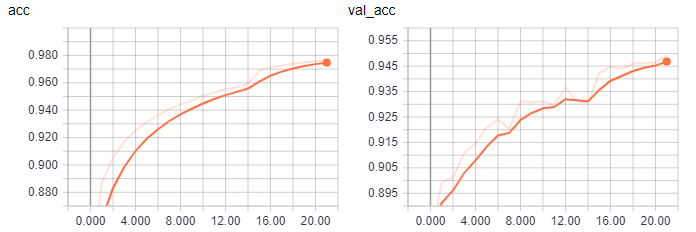
\includegraphics[width=\columnwidth]{images/acc.png}
		\caption{Accuracy improvement during training.}
		\label{fig:acc}
		\end{center}
	\end{figure}
	
	Further, table \ref{tab:scores} provides an overview about the performance on a reduced coarse grained level.
\begin{table*}[ht]
  \centering
  \caption{Performance evaluation for simplified classes.}
  \label{tab:scores}
\begin{tabular}{l|c|c|c|c|c}
	& Precision & Recall  & F1-Score   & Images  & Classes \\ 
	\hline
	\hline
	No Animal         &            0.98    &  0.99  &    0.98  &   60231 & 9 \\
	Normal $>1000$   &          0.97    &  0.97  &    0.97   &  39932 & 16 \\
	Scarce $>500$          &       0.90    &  0.69  &    0.78    &  1077 & 6 \\
	Rare $>200$              &       0.92    &  0.65 &     0.76     &  623 & 8 \\
	Very Rare $>50$      &        0.98   &   0.45 &     0.62    &   317 & 15\\
	Extremely Rare $<50$ &    0.45 &     0.28 &     0.34  &     108 & 3\\
	\hline
	\hline 
	 avg / total     &  0.97   &   0.97  &    0.97  &  102288 \\
\end{tabular}
\end{table*}

	\begin{figure}[!hbt]
		\begin{center}
		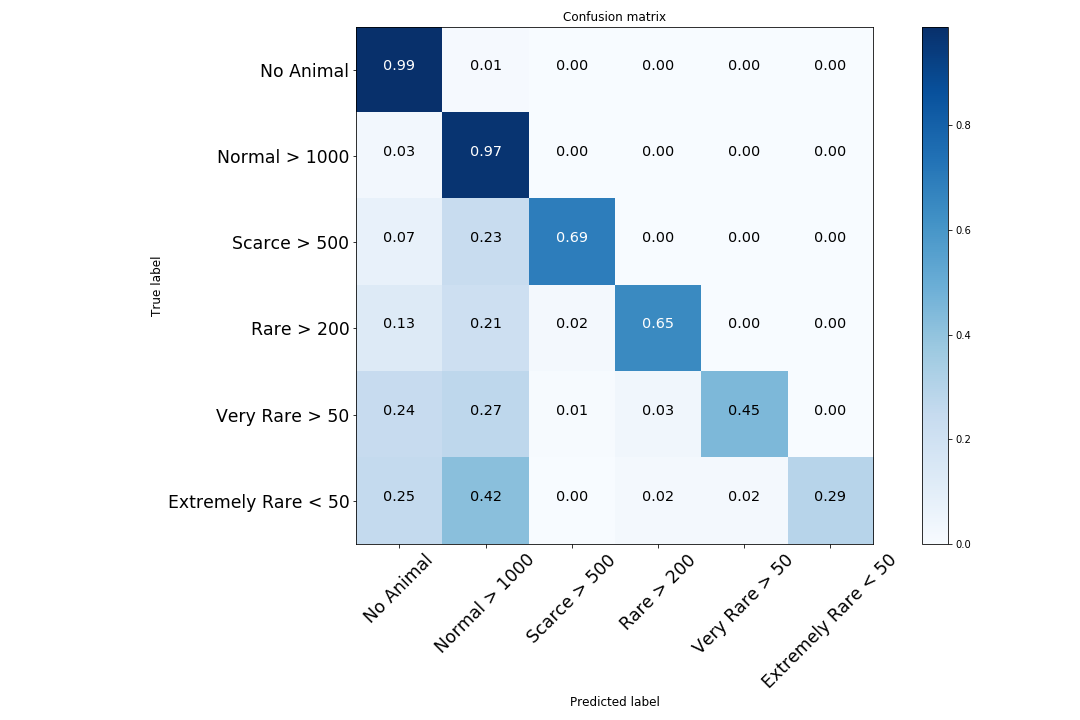
\includegraphics[width=\columnwidth]{images/conf_mat.png}
		\caption{Confusion matrix for reduced classes.}
		\label{fig:conf_mat}
		\end{center}
	\end{figure}
	

\section{Correct Attention, Correct Prediction}
	\begin{figure}[!hbt]
		\begin{center}
		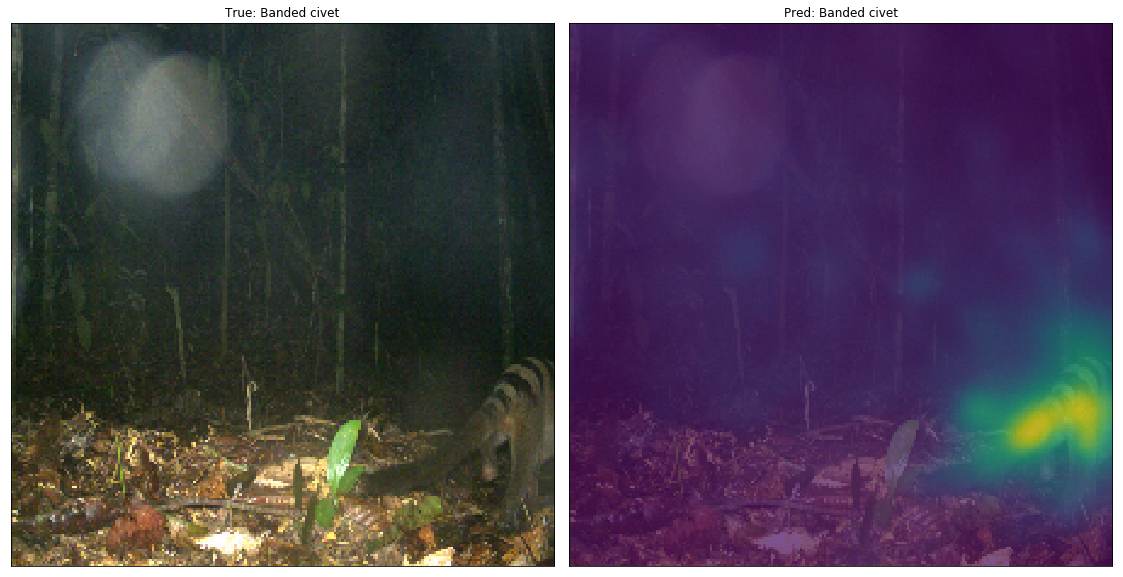
\includegraphics[width=\columnwidth]{images/good_civet.png}
		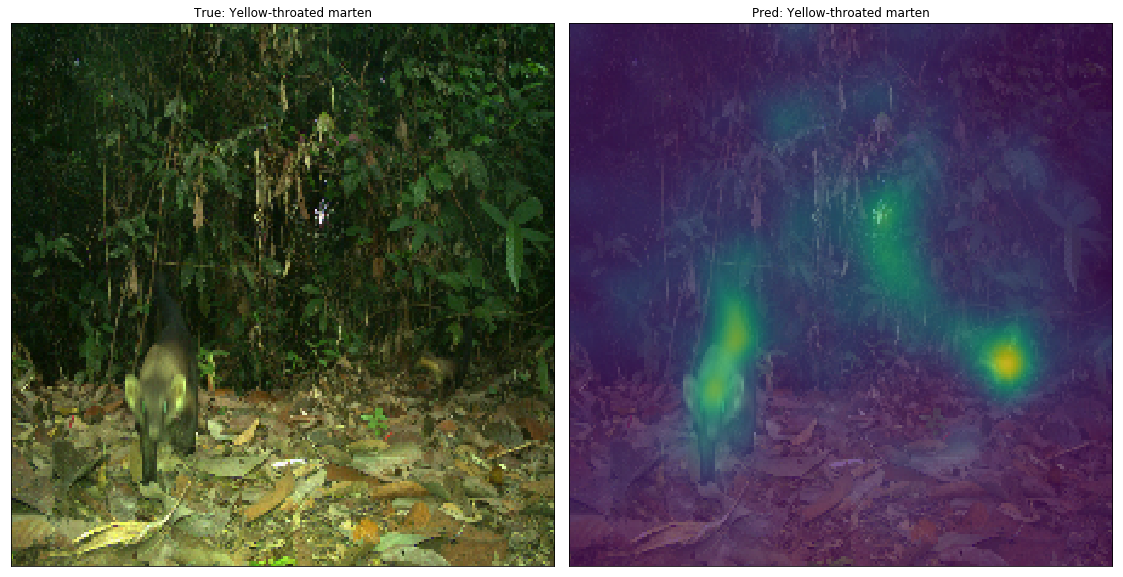
\includegraphics[width=\columnwidth]{images/Attention_right_dual.png}
		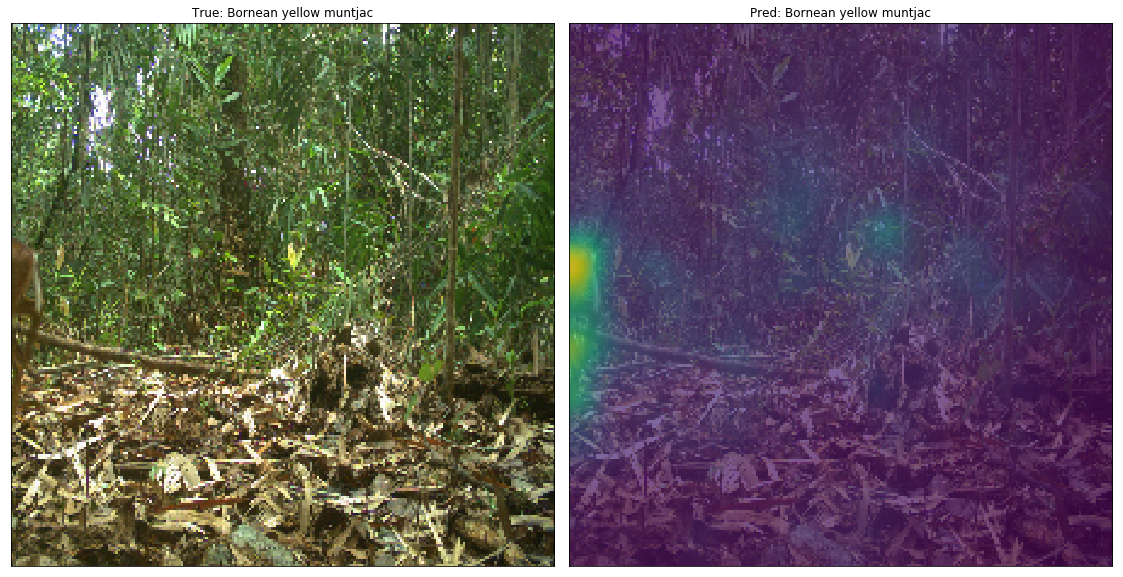
\includegraphics[width=\columnwidth]{images/Attention_right4.png}
		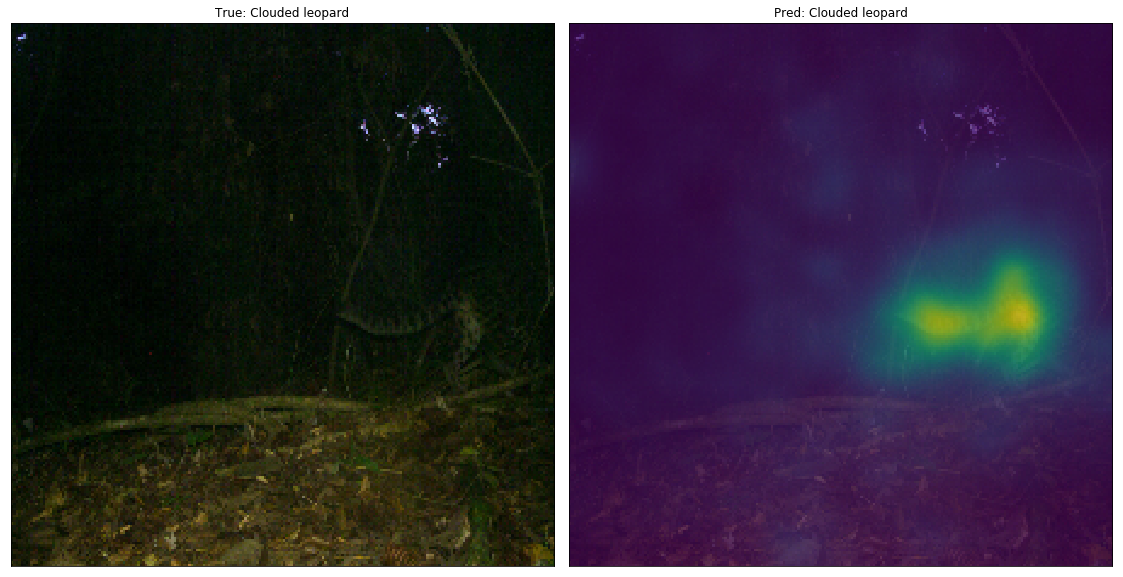
\includegraphics[width=\columnwidth]{images/Attention_right5.png}
		\caption{Correct prediction and correct attention of the network.}
		\label{fig:correct_correct}
		\end{center}
	\end{figure}

As seen in figure \ref{fig:correct_correct}  the network mainly focuses on the animal itself, this can be seen for most correct predictions. 

\section{Correct Attention, Wrong  Prediction}
	\begin{figure}[!hbt]
		\begin{center}
		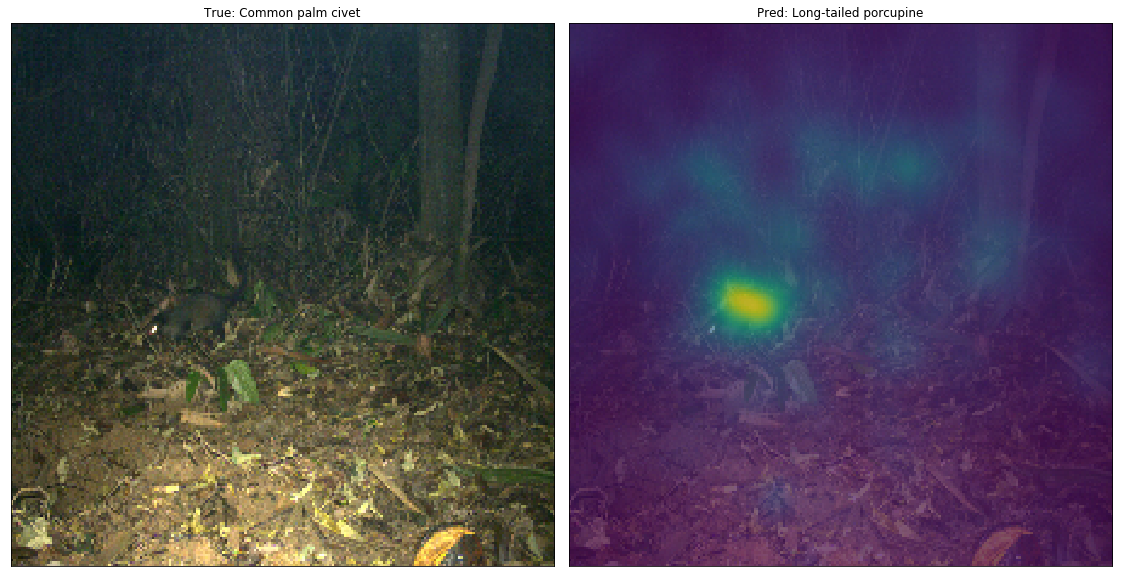
\includegraphics[width=\columnwidth]{images/Attention_wrong.png}
		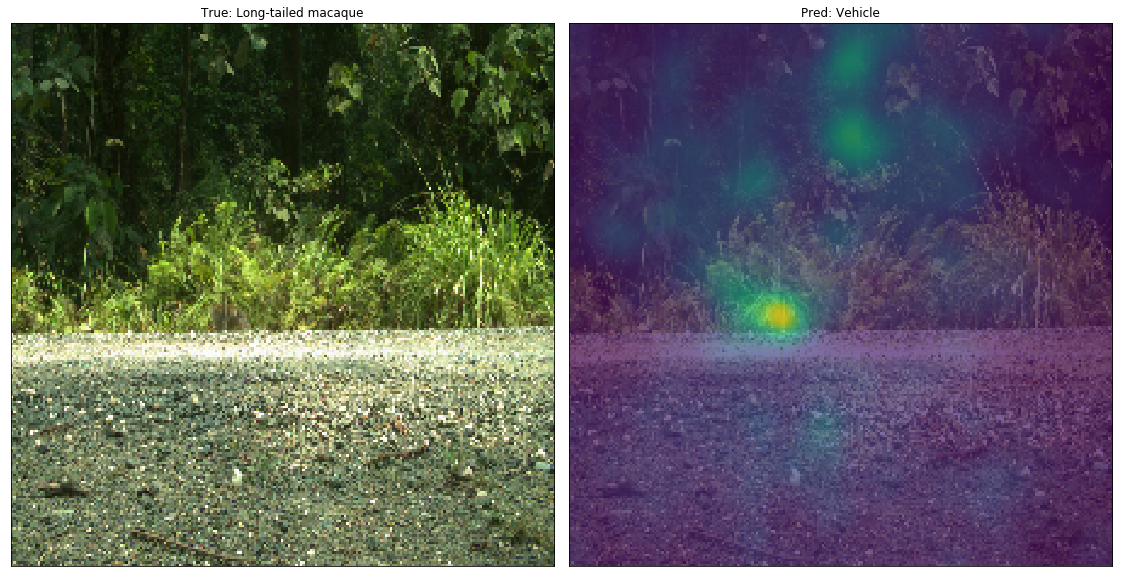
\includegraphics[width=\columnwidth]{images/Attention_wrong3.png}
		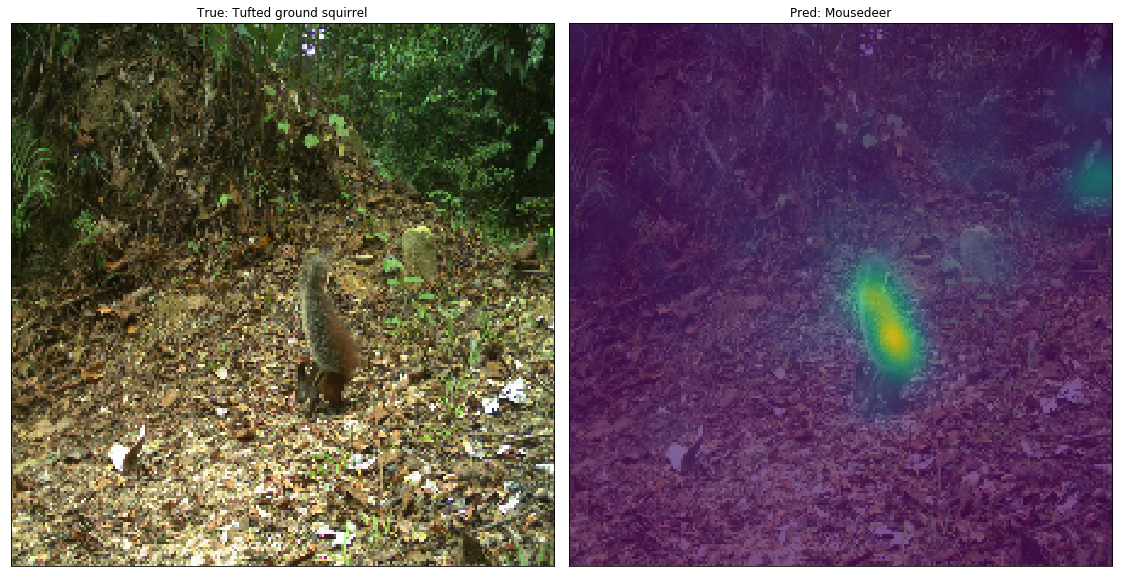
\includegraphics[width=\columnwidth]{images/Attention_wrong4.png}
		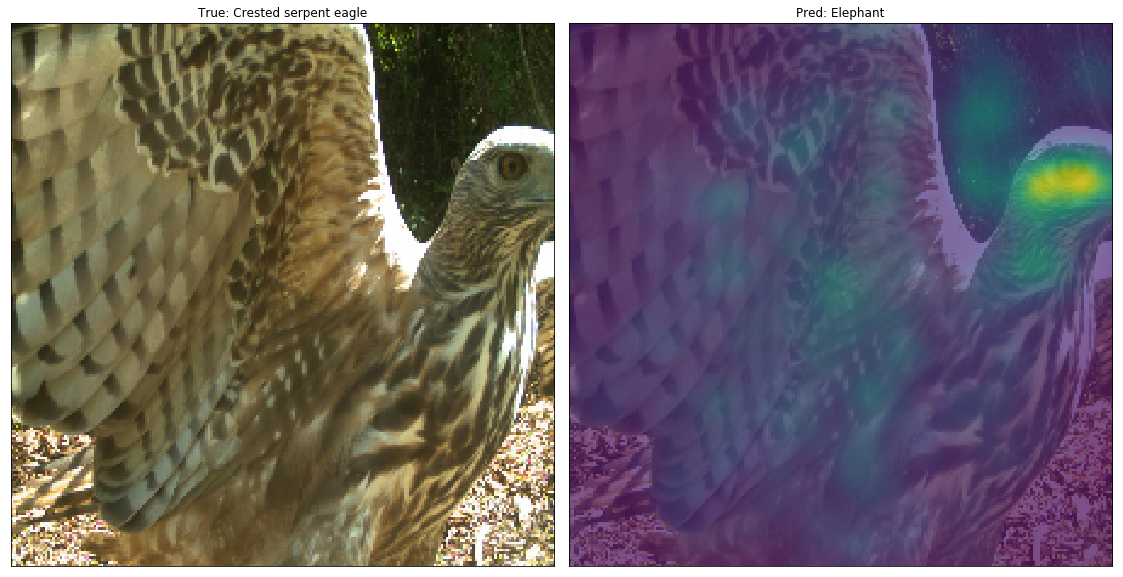
\includegraphics[width=\columnwidth]{images/Attention_wrong_easy_weird.png}
		\caption{Wrong prediction and correct attention of the network.}
		\label{fig:wrong_correct}
		\end{center}
	\end{figure}
	
The network often finds the correct attention in the images (as in \ref{fig:wrong_correct}), i.e. the animals.
However, especially rare species are still predicted incorrectly based on the small sample size during training.
This can be seen in the last image pair \ref{fig:wrong_correct}, it shows a Crested Serpent Eagle, which is classified as Elephant. 

\section{Wrong Attention, Correct Prediction}
	\begin{figure}[!hbt]
		\begin{center}
		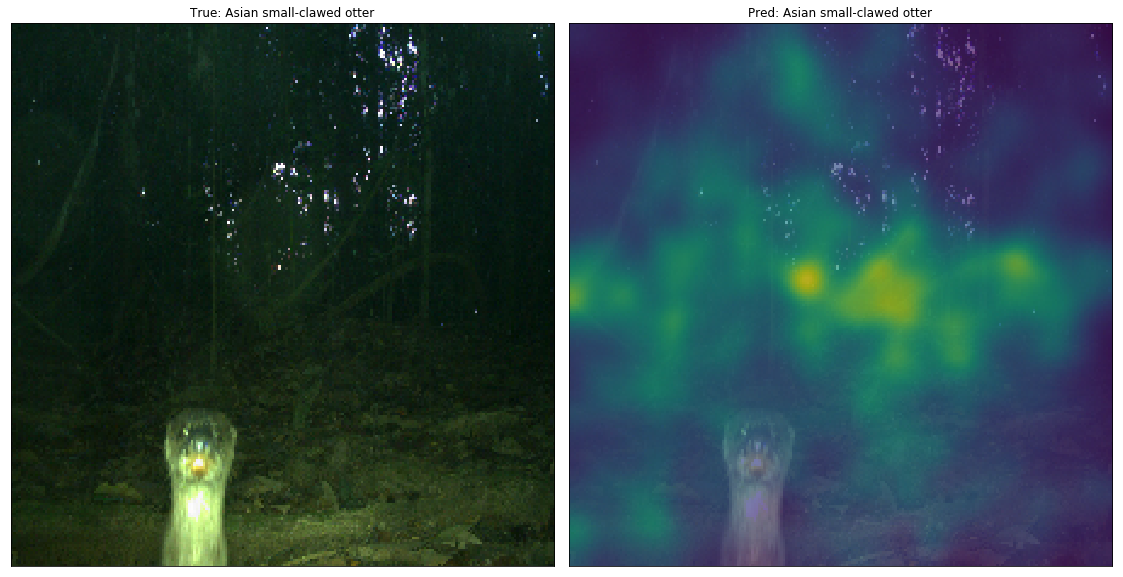
\includegraphics[width=\columnwidth]{images/No_Attention_right.png}
		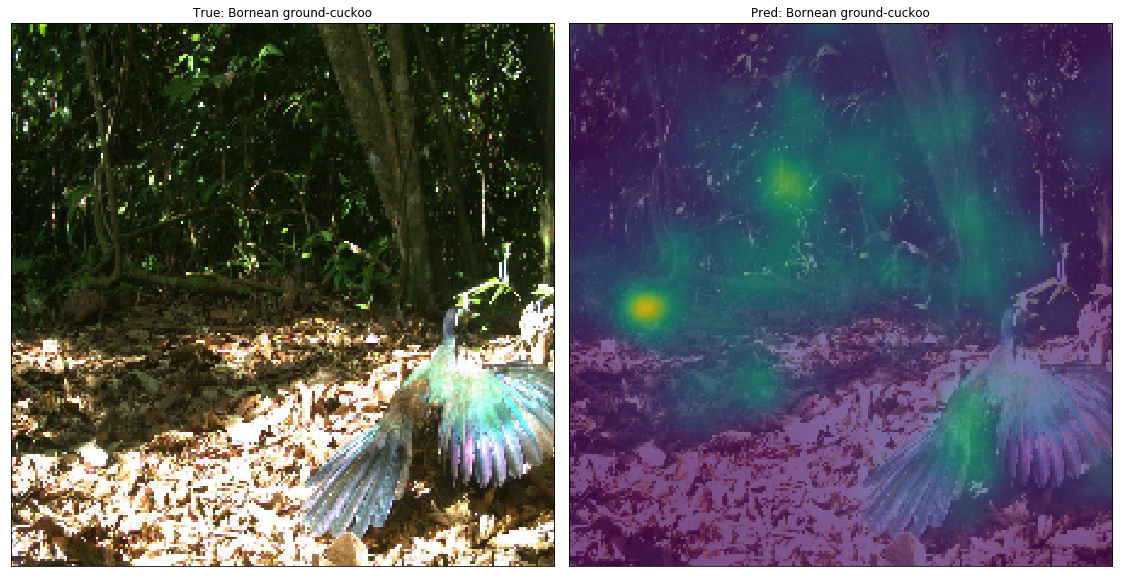
\includegraphics[width=\columnwidth]{images/No_Attention_right2.png}
		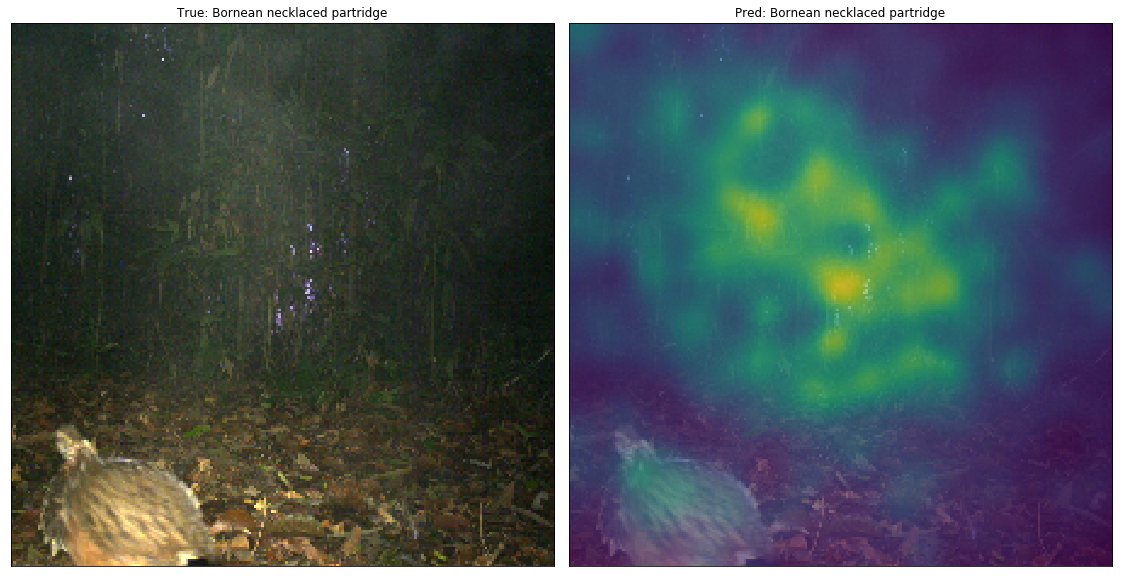
\includegraphics[width=\columnwidth]{images/No_Attention_right3.png}
		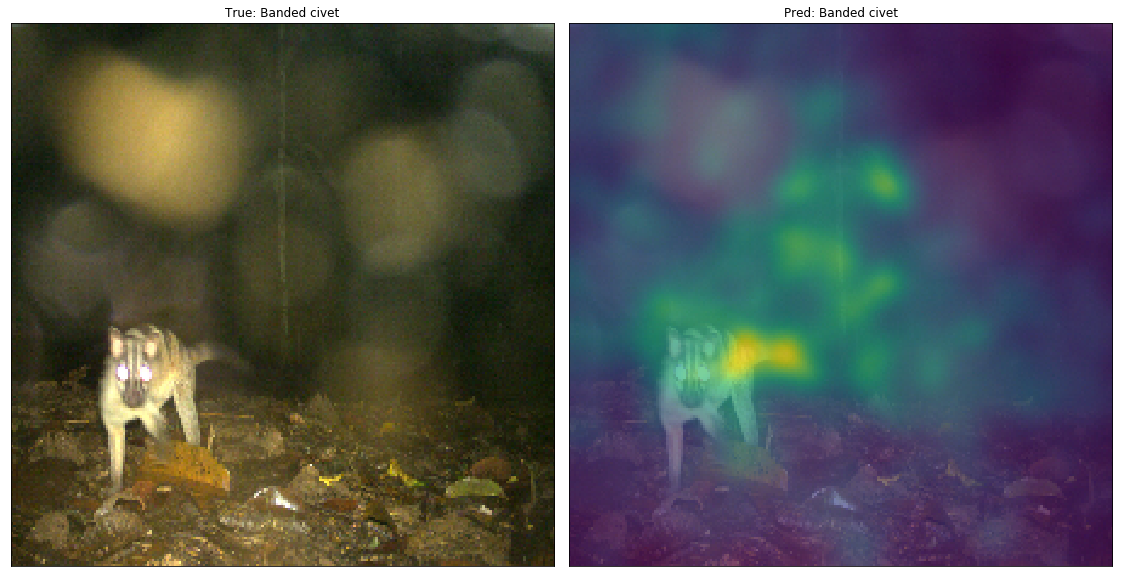
\includegraphics[width=\columnwidth]{images/Attention_Drops.png}
		\caption{Correct prediction and wrong attention of the network.}
		\label{fig:correct_wrong}
		\end{center}
	\end{figure}
	
In contrast to the first set of image from \ref{fig:correct_correct}, in some cases the attention is slightly more spread around the animal, this happens with bad lighting or similar background colors. 
This should not be seen as actual learning of the network and probably occurs due to the 3-image sequences, which are shot and provide similar context without the animal. 

\section{Wrong Attention, Wrong Prediction}
	\begin{figure}[!hbt]
		\begin{center}
		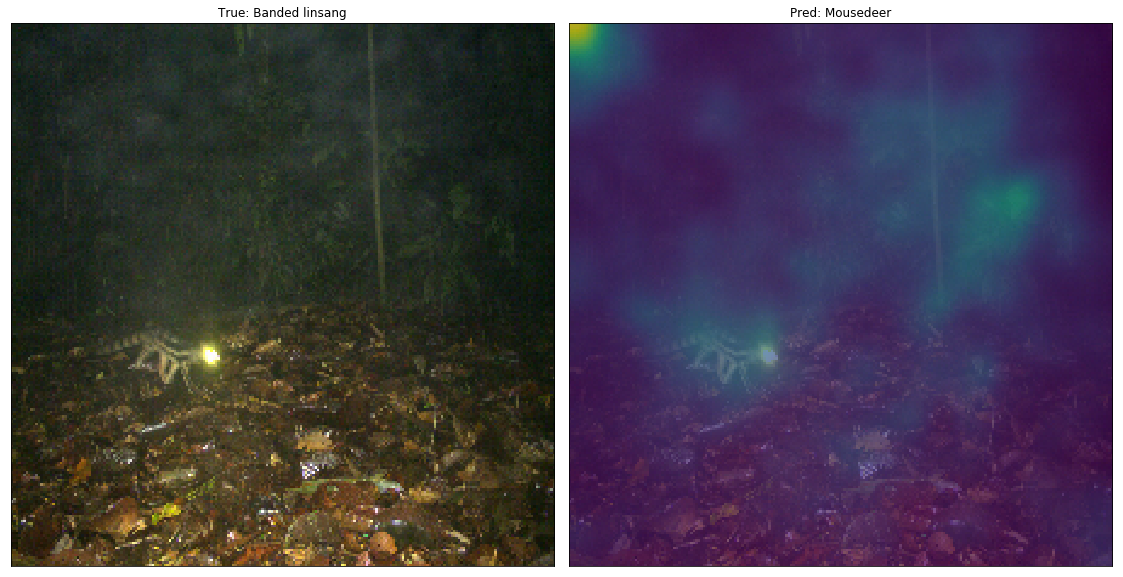
\includegraphics[width=\columnwidth]{images/No_Attention_wrong.png}
		\caption{Wrong prediction and wrong attention of the network.}
		\label{fig:wrong_wrong}
		\end{center}
	\end{figure}
	
The amount of cases in which attention and prediction are both wrong are quite limited.

\section{Notable Cases}

	\begin{figure}[!hbt]
		\begin{center}
		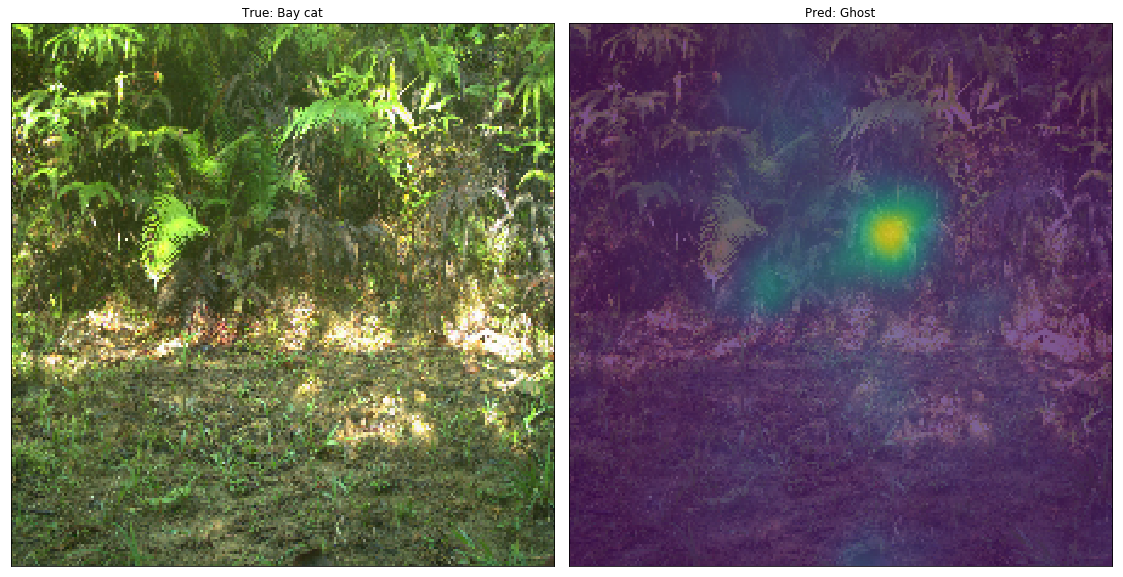
\includegraphics[width=\columnwidth]{images/No_Animal_wrong.png}
		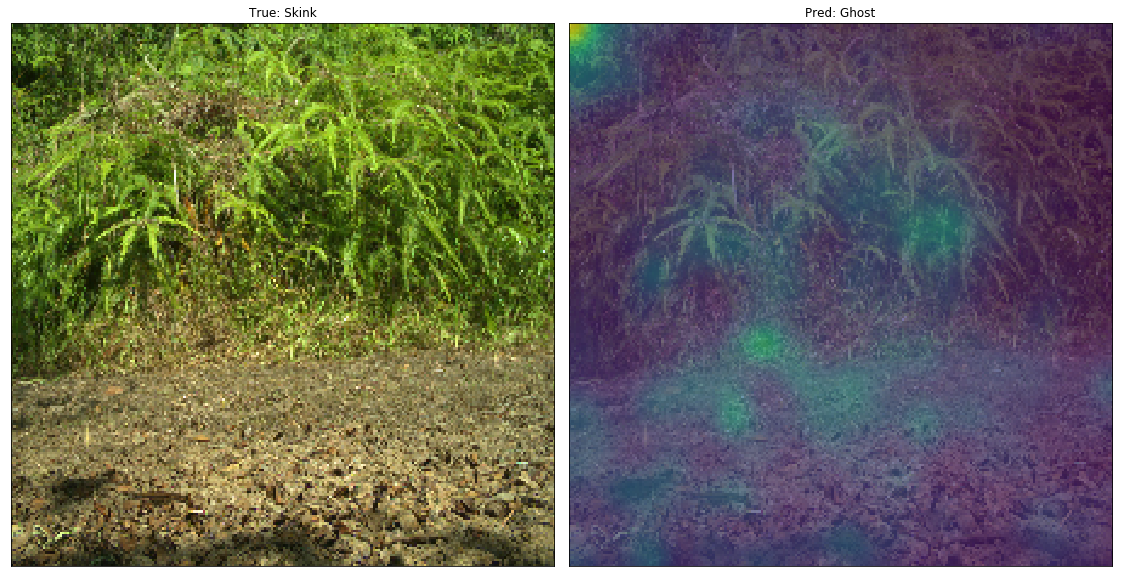
\includegraphics[width=\columnwidth]{images/No_Animal_wrong3.png}
		\caption{Wrong prediction due to noisy label (Bay Cat and Skink are actually Ghost and predicted correctly).}
		\label{fig:noisy}
		\end{center}
	\end{figure}
	\begin{figure}[!hbt]
		\begin{center}
		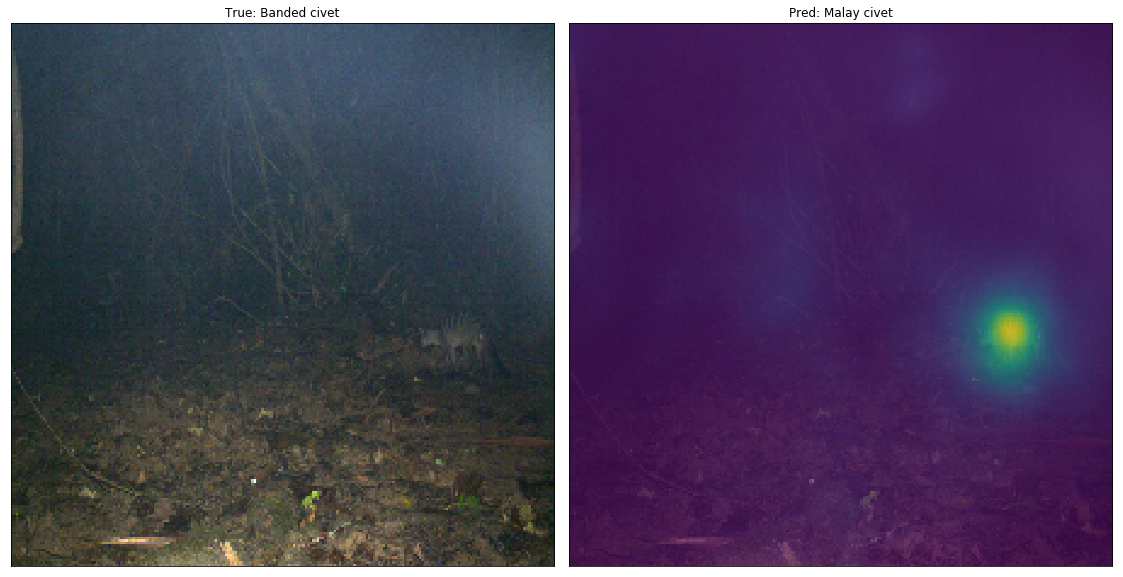
\includegraphics[width=\columnwidth]{images/mismatch.png}
		\caption{Wrong prediction due to class similarity.}
		\label{fig:mismatch}
		\end{center}
	\end{figure}

Some addtional mistakes to highlight are shown in Figure \ref{fig:mismatch} and \ref{fig:noisy}.
In figure \ref{fig:mismatch} is one example that mismatches happend due to similarities between the classes, gere specificallyÖ Banded Civet and Malay Civet.
Additionally, the provided labels include some noise, i.e. some labels might be incorrect as seen in figure \ref{fig:noisy}.
This probably can be attributed to process of taking 3-image shots and classifying all image the same. 
Besides those issues, camera occlusions due to rain are often influencing the prediction as already mentioned earlier (figure \ref{fig:correct_wrong}).
Apart from those more specific issues, as always, frequent classes are more often assigned to an incorret label, which can also be seen in the confusion matrix in figure \ref{conf_mat}.

\section{Confusion Matrix}

The reduced confusion matrix also shows that the network is able to distinguish between animals and non animals quite well as well as frequent animals, which make up the majority of the data set.
This differentiation between animals and non animals is also present for all other categories, the network is more likely to assign a wrong label from the common animal classe than from a non animal class. 

% Your document ends here!
\end{document}